\section{RESULTADOS E DISCUSSÕES}

Nesta seção será discutido, da melhor maneira possível, os resultados obtidos causando as perturbações P1-P5 no sistema de condicionamento de ar. Antes de iniciar o tópico da variação das temperaturas e pressões, é importante saber se as velocidades de rotação reais do compressor estão próximas do esperado durante o planejamento experimental. A Tabela \ref{tab:Rotações Medidas} mostra as velocidades de rotação aferidas utilizando o tacômetro MDT-2238B. Nota-se que estas velocidades estão próximas das esperadas conforme as Tabelas \ref{tab:pertubaçõesTransiente} e \ref{tab:pertubaçõesHisterese},logo, conclui-se que as condições de teste reais estão dentro do planejamento experimental esperado.

\begin{table}[htb]
    \centering
    \begin{tabular}{|c|c|}
        \hline
        \textbf{Perturbação} & \textbf{Rotação Medida no Compressor [RPM]} \\
        \hline
        P1 & 489 \\
        P2 & 838 \\
        P3 & 838 \\        
        P4 & 1083 \\
        P5 & 883 \\
        \hline
    \end{tabular}
    \caption{Velocidades de Rotação do Compressor Aferidas para as Perturbações P1-P5}
    \vspace{5pt} 
{\footnotesize Fonte: O Autor (2025) }
    \label{tab:Rotações Medidas}
\end{table}
\newpage
\subsection{\MakeUppercase{Perturbação pela Variação da Vazão de Ar do Ventilador}} \label{subsec:PertubaçãoVelVentilador}

Antes de iniciar a análise dos resultados experimentais, é importante relembrar sobre as perturbações que serão analisadas nesta subseção. As perturbações P1 e P3 são causadas pela variação da vazão de ar do ventilador do evaporador, sendo que em P1 a vazão de ar é aumentada e em P3 a vazão de ar é diminuída. Já as perturbações P2, P4 e P5 são causadas pela variação da rotação do compressor, sendo que em P2 e P4 a rotação é aumentada e em P5 a rotação é diminuída. A Tabela \ref{tab:posiçõesVentilador} relembra as perturbações causadas no sistema apresentadas na subseção \ref{subsec:PlanejamentoExperimental}.

\begin{table}[htb]
    \centering
    \begin{tabular}{|c|c|c|}
        \hline
        \textbf{Perturbação} & \makecell{\textbf{Rotação do} \\ \textbf{Compressor Esperada [RPM]}} & \textbf{Posição Ventilador}\\      
        \hline
        P1 & 500 & 1 $\rightarrow$ 4  \\
        P2 & 500 $\rightarrow$ 890 & 4  \\
        P3 & 890 & 4 $\rightarrow$ 1  \\
        P4 & 890 $\rightarrow$ 1074 & 4  \\
        P5 & 1074 $\rightarrow$ 890 & 4  \\
        \hline
    \end{tabular}
    \caption{Perturbações Geradas para Análise do Sistema}
    \vspace{5pt} 
{\footnotesize Fonte: O Autor (2025)}
    \label{tab:posiçõesVentilador}
\end{table}

A primeira observação, que talvez seja a mais específica entre todas, não observada de maneira tão clara, por exemplo, nas perturbações de rotação, são oscilações análogas a oscilações senoidais decrescentes até que o sistema estabilize em um determinado valor de temperatura ou pressão. Por exemplo, a Figura \ref{fig:TempSuccaoPertubacaoVentilador} mostra o comportamento mencionado na temperatura de sucção e descarga do compressor nas perturbações P1 e P3 apresentadas na Tabela \ref{tab:posiçõesVentilador}. As regiões de sucção e descarga estão relacionadas com a Figura \ref{fig:instalação transdutores}, onde a região de sucção é a região do transdutor de temperatura 1 e a região de descarga é a região do transdutor de temperatura 2.
\newpage
\begin{figure}[h]
    \centering
    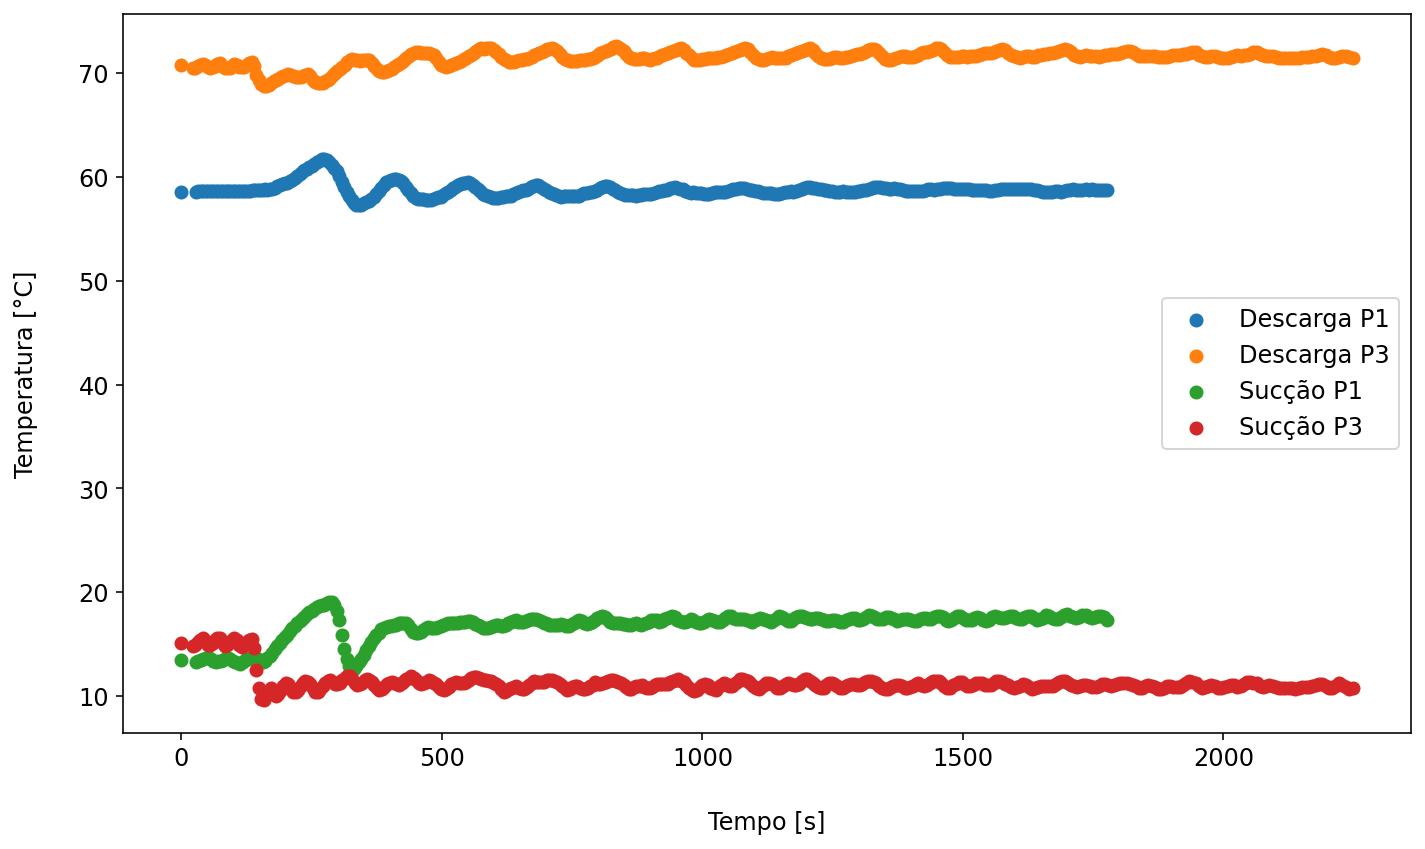
\includegraphics[width=1\linewidth]{FigurasdoTexto/Temperaturas de descarga e sucção Transiente P1 e P3.png}
    \caption{Temperaturas de Descarga e Sucção do Transiente de P1 e P3}
    \label{fig:TempSuccaoPertubacaoVentilador}
    {\footnotesize Fonte: O Autor (2025)}
\end{figure}

Nota-se, na Figura \ref{fig:TempSuccaoPertubacaoVentilador}, que há um pico máximo de temperatura de sucção e descarga em P1 logo após o aumento da vazão de ar. Este pico foi calculado como sendo 2 °C e 3 °C acima do valor final em estado estacionário das temperaturas de sucção e descarga de P1, respectivamente. Após o pico máximo, as temperaturas de sucção e descarga demoram aproximadamente 140 e 200 segundos para estabilizar em seus respectivos valores finais. Isto ocorre devido a um evaporador subalimentado \cite{StoekerRefrigeration}. Tal fato acontece quando a válvula de expansão não consegue alimentar o evaporador com refrigerante o suficiente para refrigerar a superfície do evaporador adequadamente; como resultado, a temperatura e a pressão sobem.
\newpage
O pico mínimo de temperatura ocorre logo depois, provavelmente, devido a um evaporador inundado, isto é, após a subalimentação do evaporador, a válvula de expansão então deixa que mais fluido refrigerante passe até que o evaporador inunde, esta interpretação pode ser embasada com dados experimentais como na Figura \ref{fig:VazãodeFluidoPerturbaçãoVentilador}, onde há um pico máximo de vazão de fluido refrigerante ao mesmo tempo em que as temperaturas de sucção e descarga são mínimas. Além disso, no artigo de \textcite{VaryingFanSpeedCavallaro} foi observado que aumentar a vazão de ar do ventilador implica em um aumento do coeficiente de transferência de calor h do sistema. Isto também deve estar auxiliando para que a queda da temperatura ocorra mais rapidamente.

\begin{figure}[h]
    \centering
    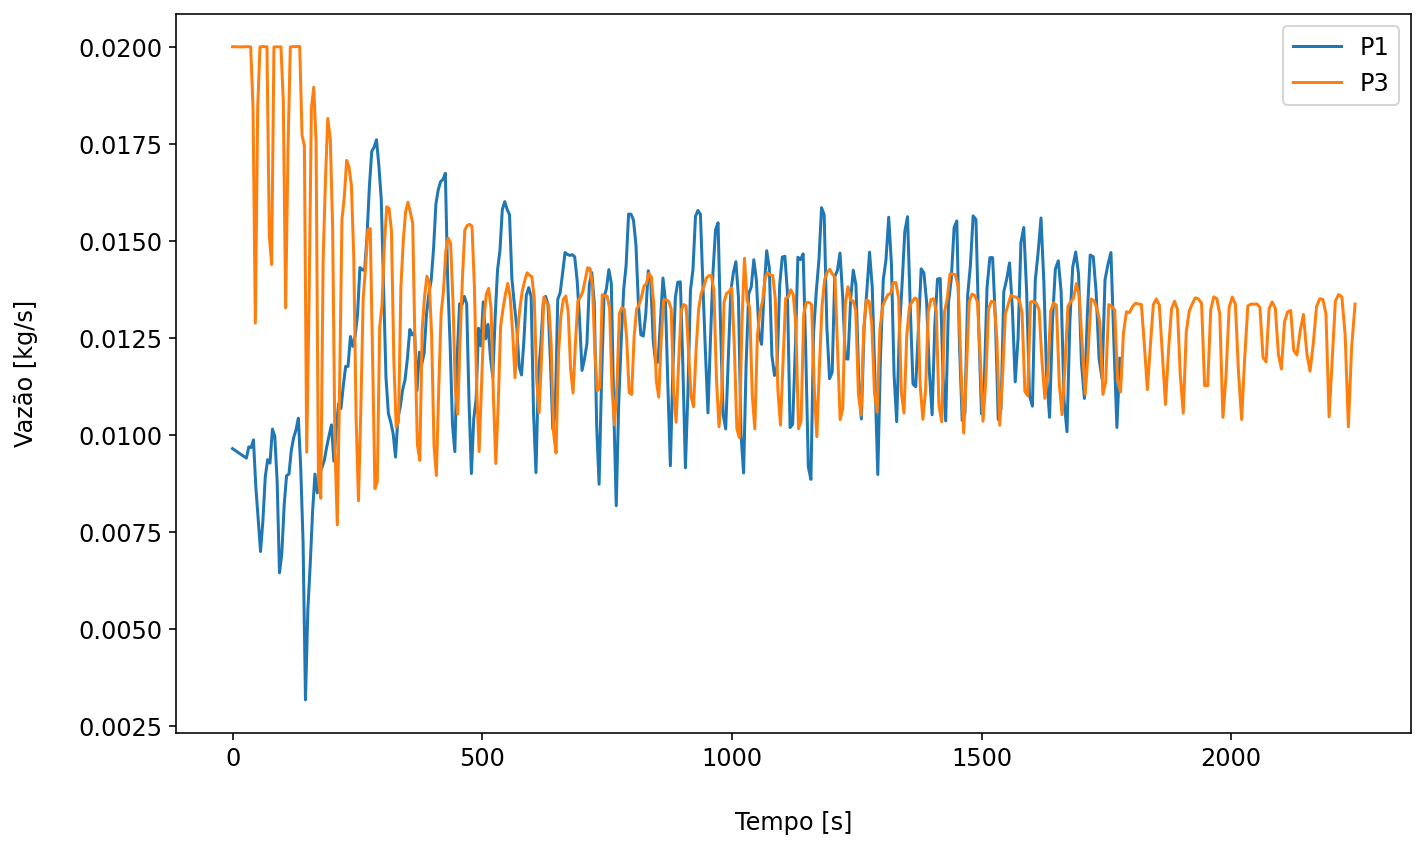
\includegraphics[width=1\linewidth]{FigurasdoTexto/VazãodeFluidoPerturbaçãoVentilador.png}
    \caption{Vazão de Fluido Refrigerante Transiente de P1 e P3}
    \label{fig:VazãodeFluidoPerturbaçãoVentilador}
    {\footnotesize Fonte: O Autor (2025)}
\end{figure}
%Explicações- as temperaturas atingem um pico máximo devido a um evaporador seco (stoeker) causando aumento de temperatura e pressão e um pico mínimo de fluido vazão de fluido refrigerante. Já o mínimo ocorre devido a um evaporador cheio (inundado), faz sentido porque há um pico de vazão de fluido refrigerante .

No entanto, as temperaturas de sucção e descarga após isso sobem aproximadamente 5 °C  e 1 °C, respectivamente, em relação à temperatura mínima atingida, e oscilam até estabilizar. Esta subida de temperatura possivelmente tem relação com que, embora o coeficiente de transferência de calor tenha aumentado, há mais vazão de ar do que o que pode ser resfriado de maneira mais eficaz pelo sistema, então as temperaturas sobem e fazem isso oscilando, procurando a posição de equilíbrio entre a pressão de sucção e o fluxo da taxa de massa \cite{StoekerRefrigeration}.  
\newpage
No caso de P3 não são observados extremos de temperatura, provavelmente pois, como a velocidade e vazão de ar neste caso são reduzidos, diminuí-los é uma alteração menos brusca no sistema, ela apenas decresce oscilando, devido possivelmente à mesma razão que P1 cresce, isto é, com menos vazão de ar é mais fácil resfriá-lo e oscila procurando o equilíbrio.

As pressões de descarga e sucção ambas crescem ou decrescem conjuntamente, o que é o oposto do observado nas pressões nas perturbações por rotação. Como na Figura \ref{fig:Pressões de Sucção e Descarga P1 e P3}, o aumento das pressões ou a diminuição delas ocorre em decorrência do aumento ou diminuição da carga térmica no evaporador, respectivamente \cite{EffectsOFRefrigeranteCompressorAirFlow}.

\begin{figure}[h]
    \centering
    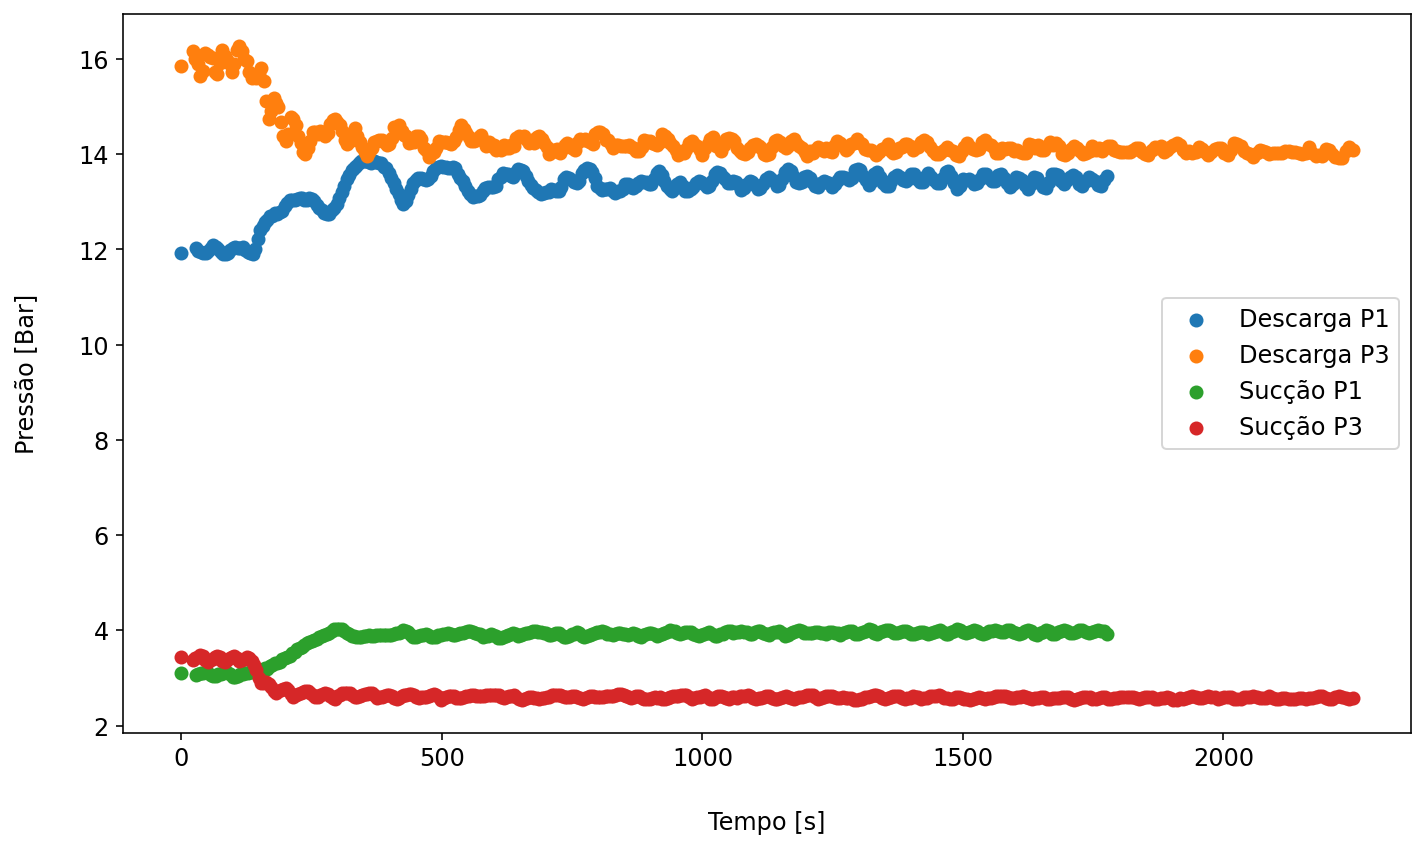
\includegraphics[width=1\linewidth]{FigurasdoTexto/Pressões de Sucção e Descarga P1 e P3.png}
    \caption{Pressões de Descarga e Sucção P1 e P3}
    \label{fig:Pressões de Sucção e Descarga P1 e P3}
    {\footnotesize Fonte: O Autor (2025)}
\end{figure}
\newpage
\subsection{\MakeUppercase{Perturbação pela Variação de Rotação do Compressor}}\label{subsec:PertubaçãoRotacaoCompressor}


As perturbações causadas por rotação, como P2, P4 e P5, demonstraram um comportamento, em geral, menos oscilatório do que as que foram apresentadas previamente na subseção \ref{subsec:PertubaçãoVelVentilador}. É perceptível que, em relação às pressões, quando há aumento da velocidade de rotação do compressor, a pressão de descarga sobe aproximadamente 3 bar e a de sucção desce cerca de 1 bar. Esta relação inversa entre as pressões também foi apontada em outros trabalhos, como o estudo de \textcite{EffectsOFRefrigeranteCompressorAirFlow}. Por exemplo, a Figura \ref{fig:Pressão de Descarga e Sucção P2} mostra esta relação nas pressões de P2. 

\begin{figure}[h]
    \centering
    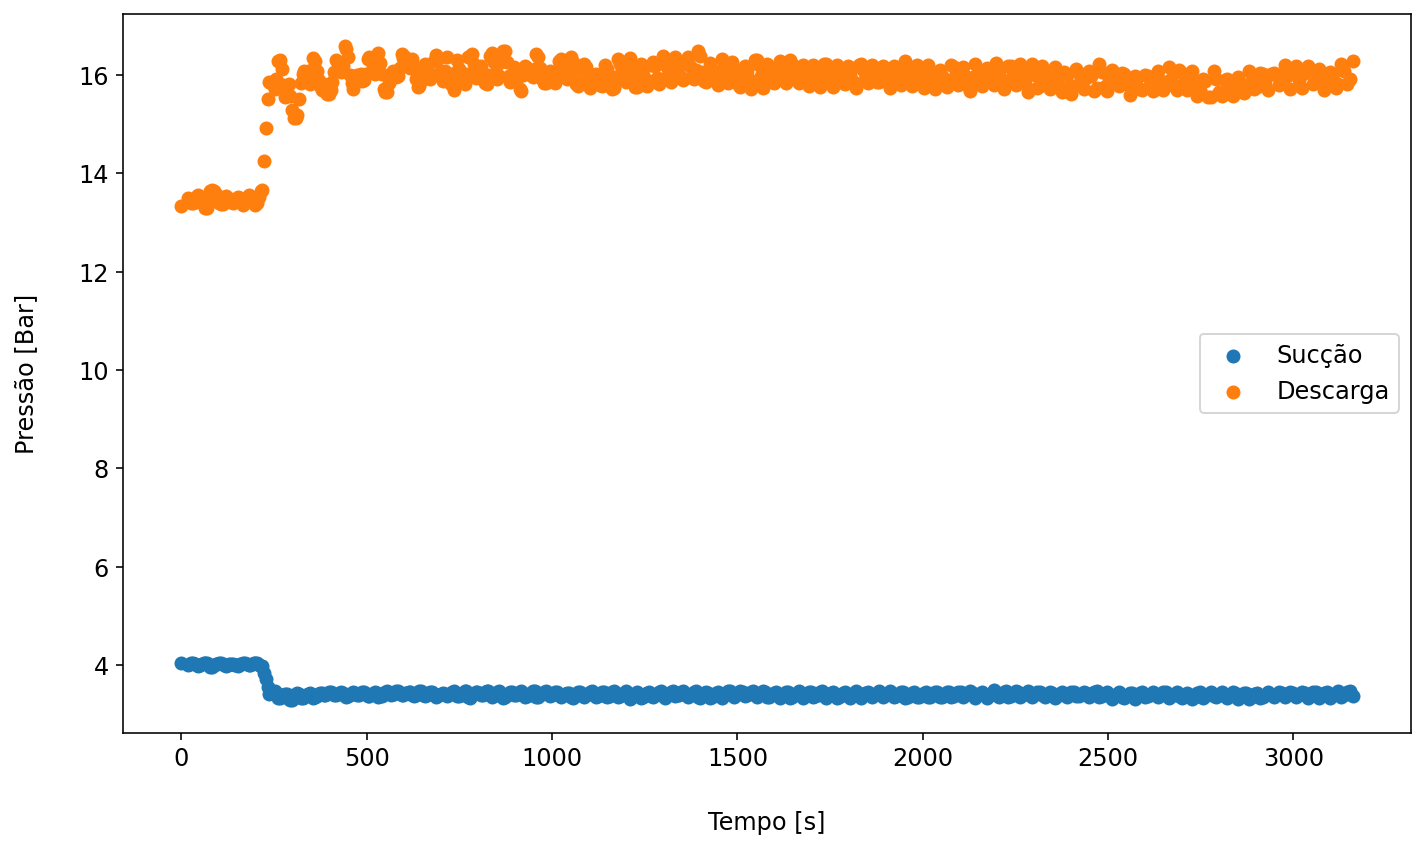
\includegraphics[width=1\linewidth]{FigurasdoTexto/Pressão de Descarga e Sucção P2.png}
    \caption{Pressões de Descarga e Sucção P2}
    \label{fig:Pressão de Descarga e Sucção P2}
    {\footnotesize Fonte: O Autor (2025)}
\end{figure}

A relação inversa entre as pressões pode ser explicada devido à capacidade do compressor aumentar quando a rotação é elevada, variando então inversamente as quedas de pressão, como pode ser representado por um diagrama P-V do compressor, as quedas de pressão variam com o RPM ao quadrado \cite{phillippi2008basic}.
É observado também uma maior variação na pressão de descarga do que na pressão de sucção; tal comportamento ocorre devido ao aumento da região ocupada por líquido sub-resfriado no condensador. A prática é usual e serve à função de fazer com que apenas líquido entre na válvula de expansão \cite{StoekerRefrigeration}.

O transiente da parte de sucção é mais rápido que na parte de descarga e isto é possível de concluir não somente das pressões, mas também das temperaturas respectivas, assim como mostra a Figura \ref{fig:Temperaturas de Sucção e Descarga P2}. Esta diferente velocidade dos transientes ocorre, provavelmente,devido à maior inércia térmica do condensador, fazendo com que a sua resposta seja mais lenta e também devido ao efeito da válvula de expansão. Ao aumentar a velocidade do compressor, a carga térmica aumenta quase que instantaneamente no sistema, isto aumenta a pressão e temperatura de descarga e mais  fluido refrigerante é sugado pelo compressor por consequência. No entanto, a válvula de expansão ainda demora para permitir que mais fluido refrigerante passe para o evaporador \cite{CHEN20081368}. Então, causando atraso, como visto nas Figuras \ref{fig:Pressão de Descarga e Sucção P2} e \ref{fig:Temperaturas de Sucção e Descarga P2}. 

\begin{figure}[h]
    \centering
    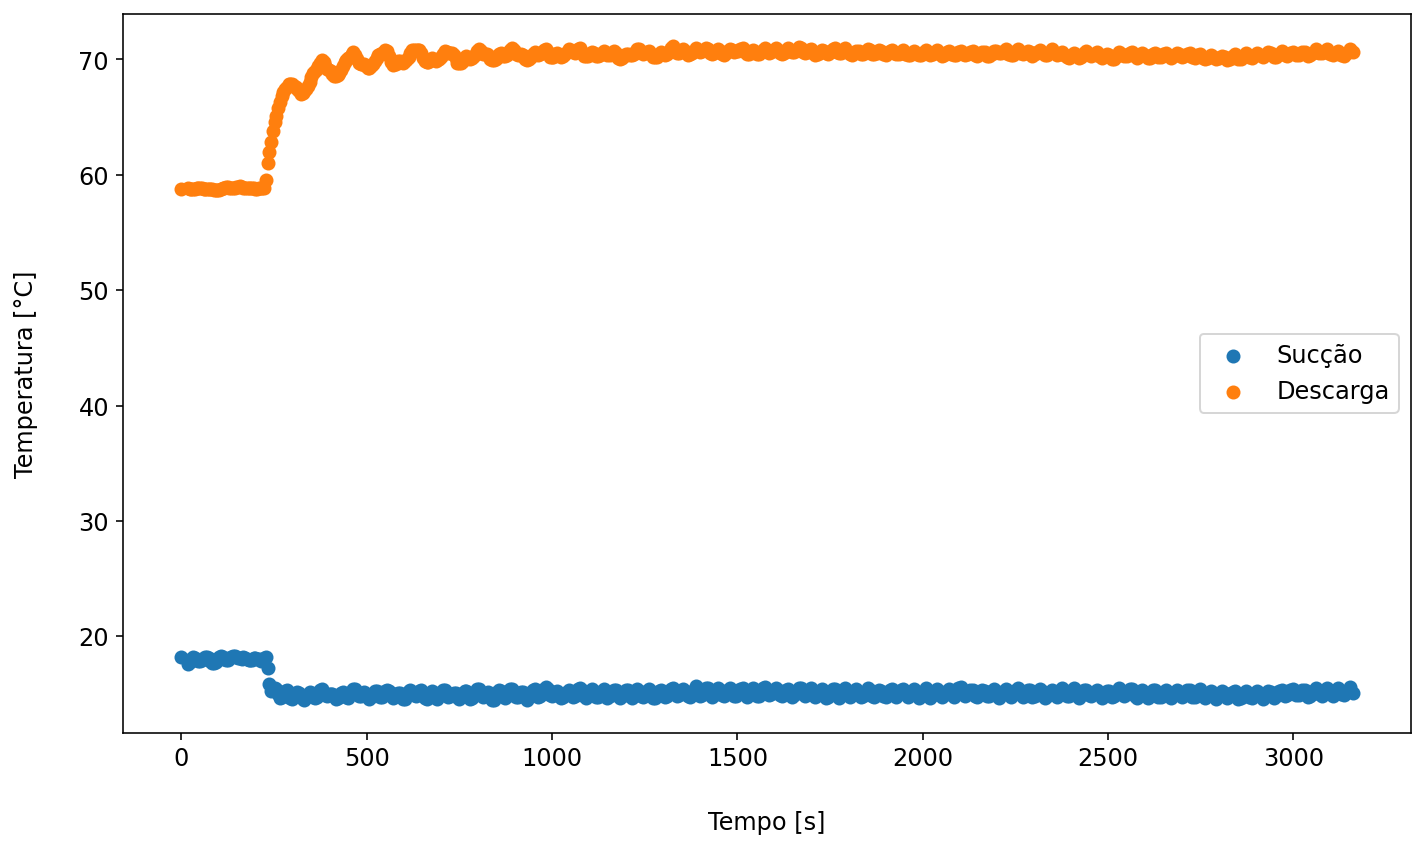
\includegraphics[width=1\linewidth]{FigurasdoTexto/Temperaturas de Sucção e Descarga P2.png}
    \caption{Temperaturas de Descarga e Sucção P2}
    \label{fig:Temperaturas de Sucção e Descarga P2}
    {\footnotesize Fonte: O Autor (2025)}
\end{figure}
%\subsection{Estimativa dos Tempos de Acomodação}\newpage
\newpage
\subsection{\MakeUppercase{Análise da Histerese}}

 Os resultados obtidos são calculados a partir das variáveis das perturbações P4 e P5, cujo teste foi realizado de forma que a rotação do compressor voltasse ao seu estado inicial, permitindo desta forma aferir a histerese, conforme anteriormente apresentado nas Tabelas \ref{tab:pertubaçõesHisterese} e \ref{tab:posiçõesVentilador} utilizando o método de análise introduzido na subseção \ref{subsec:Método de Análise da Histerese} deste trabalho. A Figura \ref{fig:histereses normalizadas} demonstra, então, esses valores encontrados.

 \begin{figure}[h] 
%gráfico a rever devido a valores maiores de histerese não antes analisados, mas creio que deve ter a ver com o que o lôndero falou da demora/rapidez conforme a mudança da válvula de expansão

%valores agora estão mais realistas, o problema é que estava comparando a entra e saída do 1002 com o 1001 e 1002 com 1004 o que não fazia sentido
    \centering
    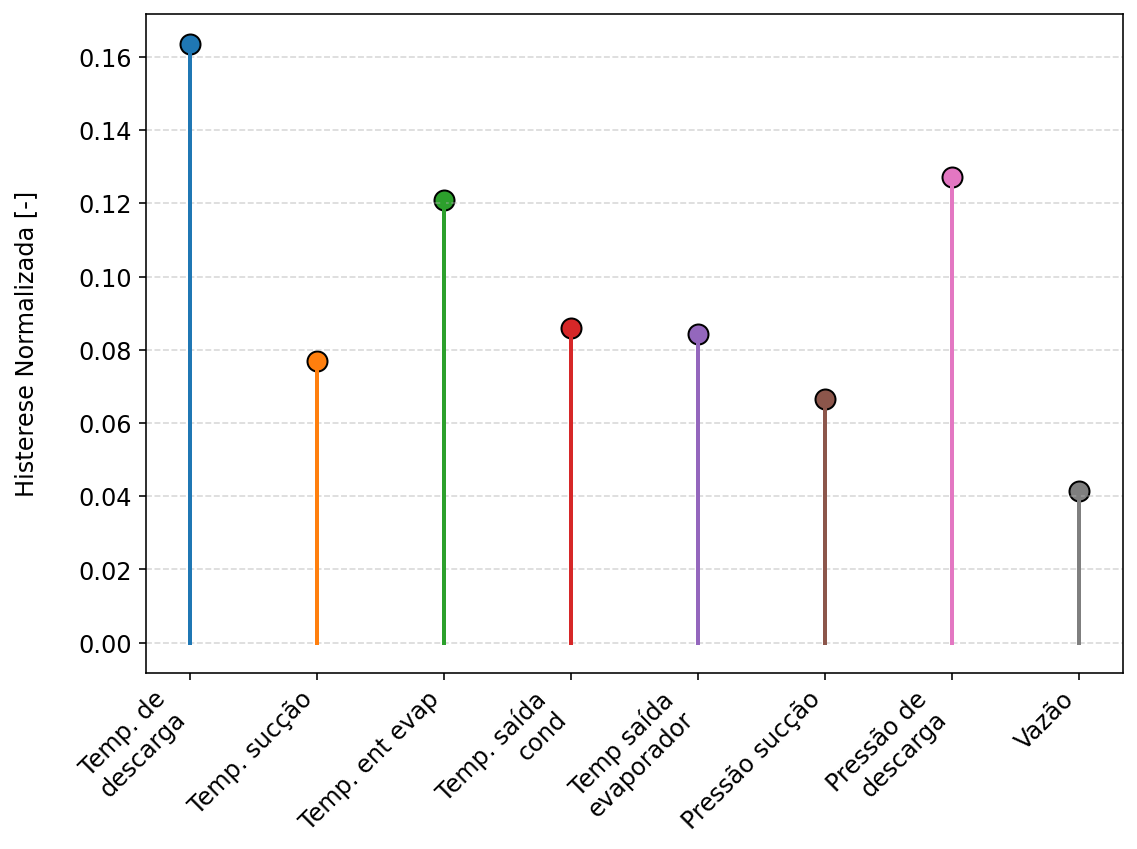
\includegraphics[width=1\linewidth]{FigurasdoTexto/Histereses Normalizadas.png}
    \caption{Histereses Normalizadas das Principais Variáveis do Teste}
    \label{fig:histereses normalizadas}
    {\footnotesize Fonte: O Autor (2025)}
\end{figure}

Nota-se que as histereses mais altas, como observadas na Figura \ref{fig:histereses normalizadas} sendo Temp. de descarga e Pressão de descarga, encontram-se próximas da região da válvula de expansão. O que é um possível indício de que ela é a principal responsável pelas variações observadas no sistema, como, por exemplo, a diferença entre a velocidade dos transientes das variáveis de P4 e P5. É também perceptível que a velocidade de convergência das variáveis de teste é afetada pela subida ou descida de rotação, principalmente das de menor histerese, como a temperatura e pressão de sucção. Por exemplo, o gráfico da Figura \ref{fig:PressãodeSucçãoSubidaeDescida} mostra a pressão de sucção nas perturbações P4 e P5, nota-se que em boa parte do transiente na subida de rotação há uma lacuna na coleta dos dados. Isto acontece pois a subida do transiente foi mais rápida do que a taxa de amostragem do sistema de aquisição.

\begin{figure}[h]
    \centering
    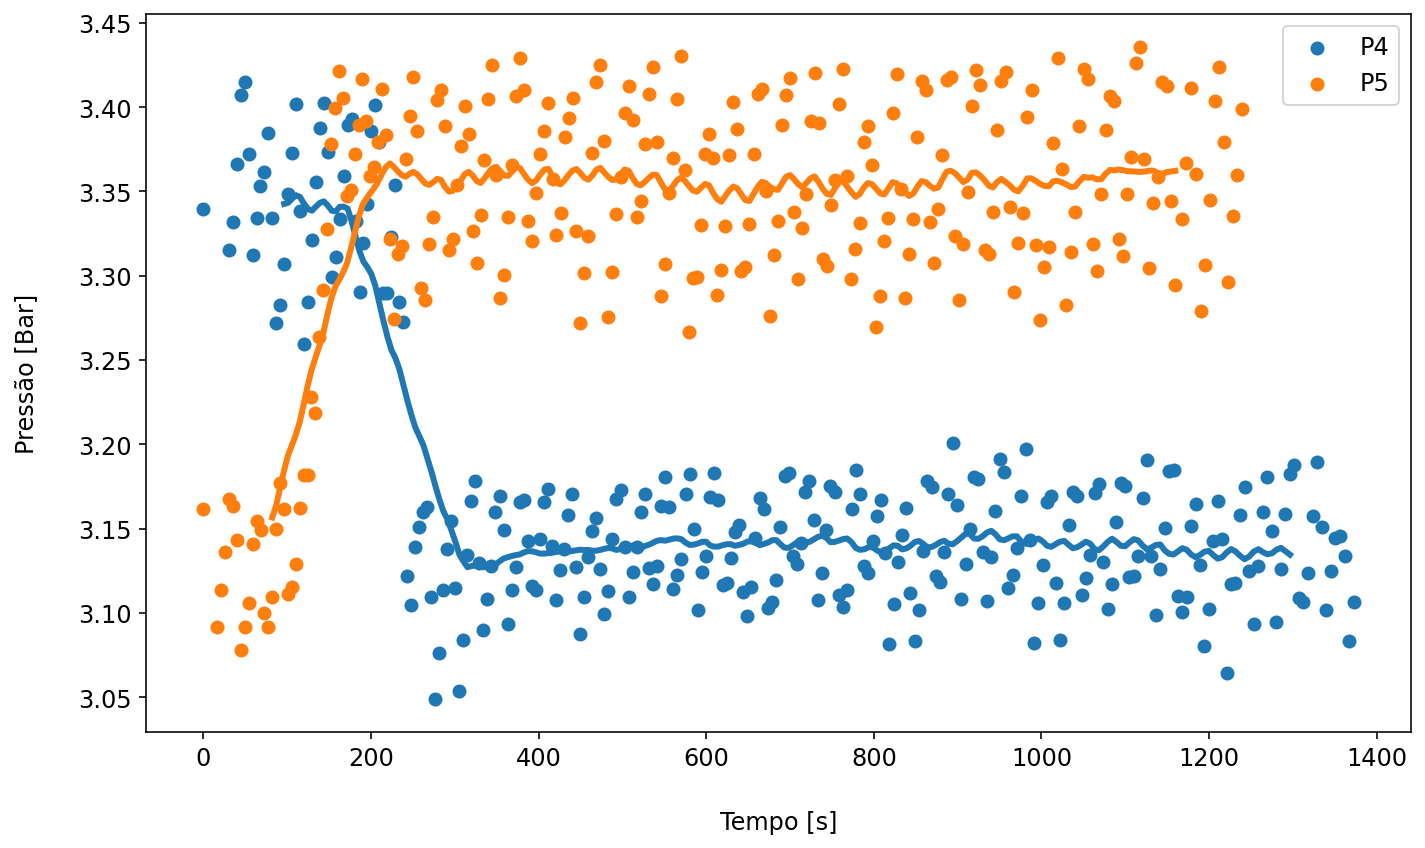
\includegraphics[width=1\linewidth]{FigurasdoTexto/Pressão de sucção subida e descida1.png}
    \caption{Pressão de Sucção nas Perturbações P4 e P5}
    \label{fig:PressãodeSucçãoSubidaeDescida}
    {\footnotesize Fonte: O Autor (2025)}
\end{figure}

Uma possível explicação para esta mudança da velocidade de convergência pode ser o efeito da válvula de expansão. Quando a velocidade de rotação do compressor é diminuída, a vazão de fluido refrigerante passando pela válvula diminui, então ela começa a se fechar, não completamente, mas há diminuição da seção por onde passa o fluido, causando atraso no aumento da pressão de sucção. Contrastando com a situação oposta, isto é, durante o aumento da velocidade de rotação, há um aumento na vazão de fluido refrigerante, e a válvula já está completamente aberta, permitindo que a pressão varie mais facilmente. Tal comportamento é observável não só na pressão de sucção, mas também na temperatura, como mostra a Figura \ref{fig:TempSucçãoSubidaeDescida}, o que demonstra que o comportamento citado acima é compatível com a observação experimental.
\newpage
\begin{figure}[h]
    \centering
    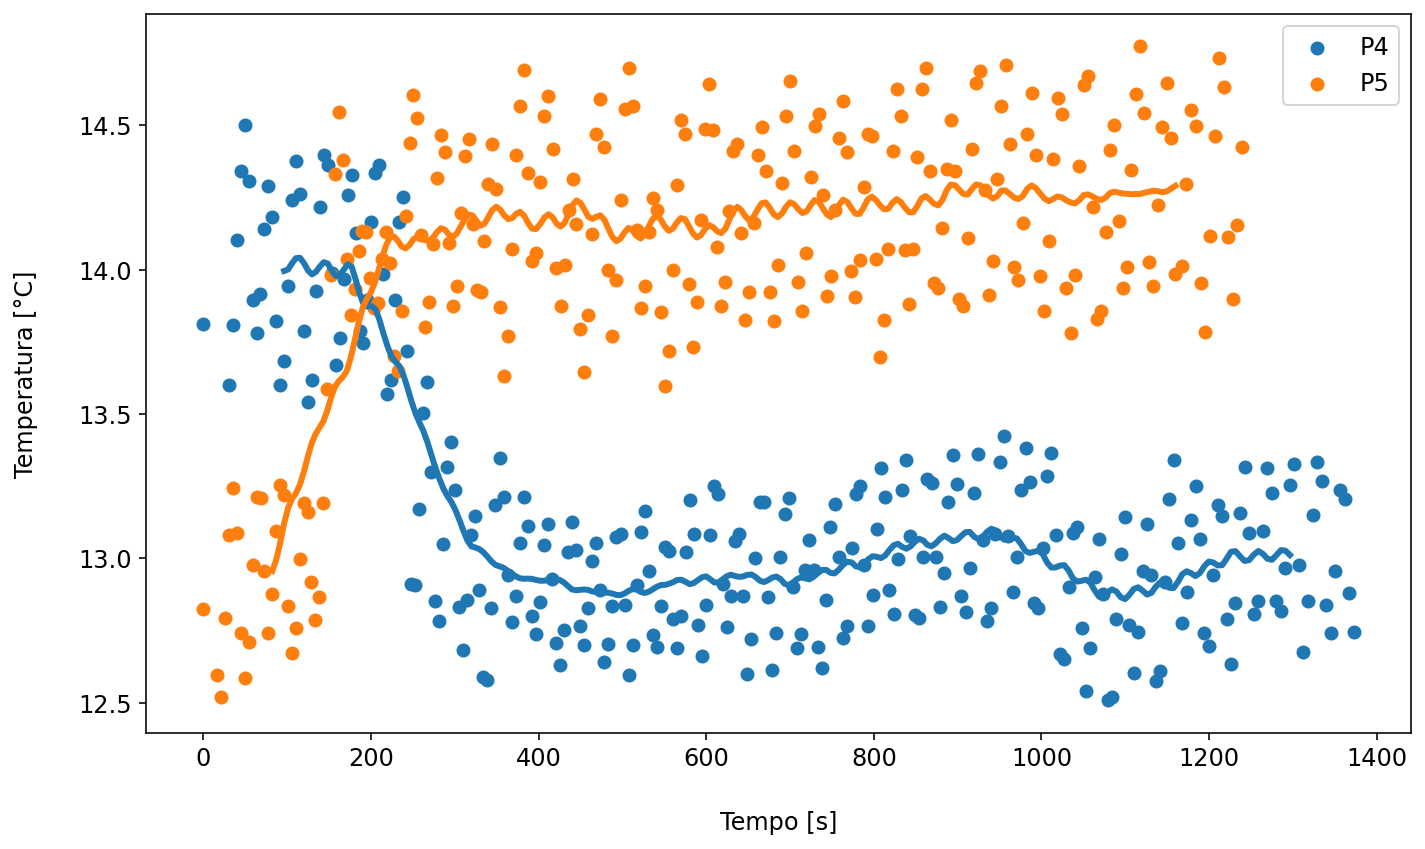
\includegraphics[width=1\linewidth]{FigurasdoTexto/Temperatura de Sucçãohyst.png}
    \caption{Temperatura de Sucção  nas Perturbações P4 e P5}
    \label{fig:TempSucçãoSubidaeDescida}
    {\footnotesize Fonte: O Autor (2025)}
\end{figure}

O transiente da pressão e temperatura de descarga é mais lento que o de sucção, como demonstrado na Figura \ref{fig:TempDescargaSubidaeDescida}. O que já era esperado, conforme discutido na subseção \ref{subsec:PertubaçãoRotacaoCompressor} de forma mais detalhada.
Percebe-se, no entanto, após a estabilização da temperatura de descarga em P5, ela não volta ao mesmo valor que tinha inicialmente em P4, o que deveria ser o comportamento esperado. É razoável propor que isso ocorra devido ao aumento da temperatura ambiente, que foi de 22 °C em P4 para 24 °C ao final de P5, o que diminui a eficiência do sistema de condicionamento de ar e, consequentemente, a temperatura de descarga não conseguiu voltar ao seu valor inicial.
\newpage
\begin{figure}[h]
    \centering
    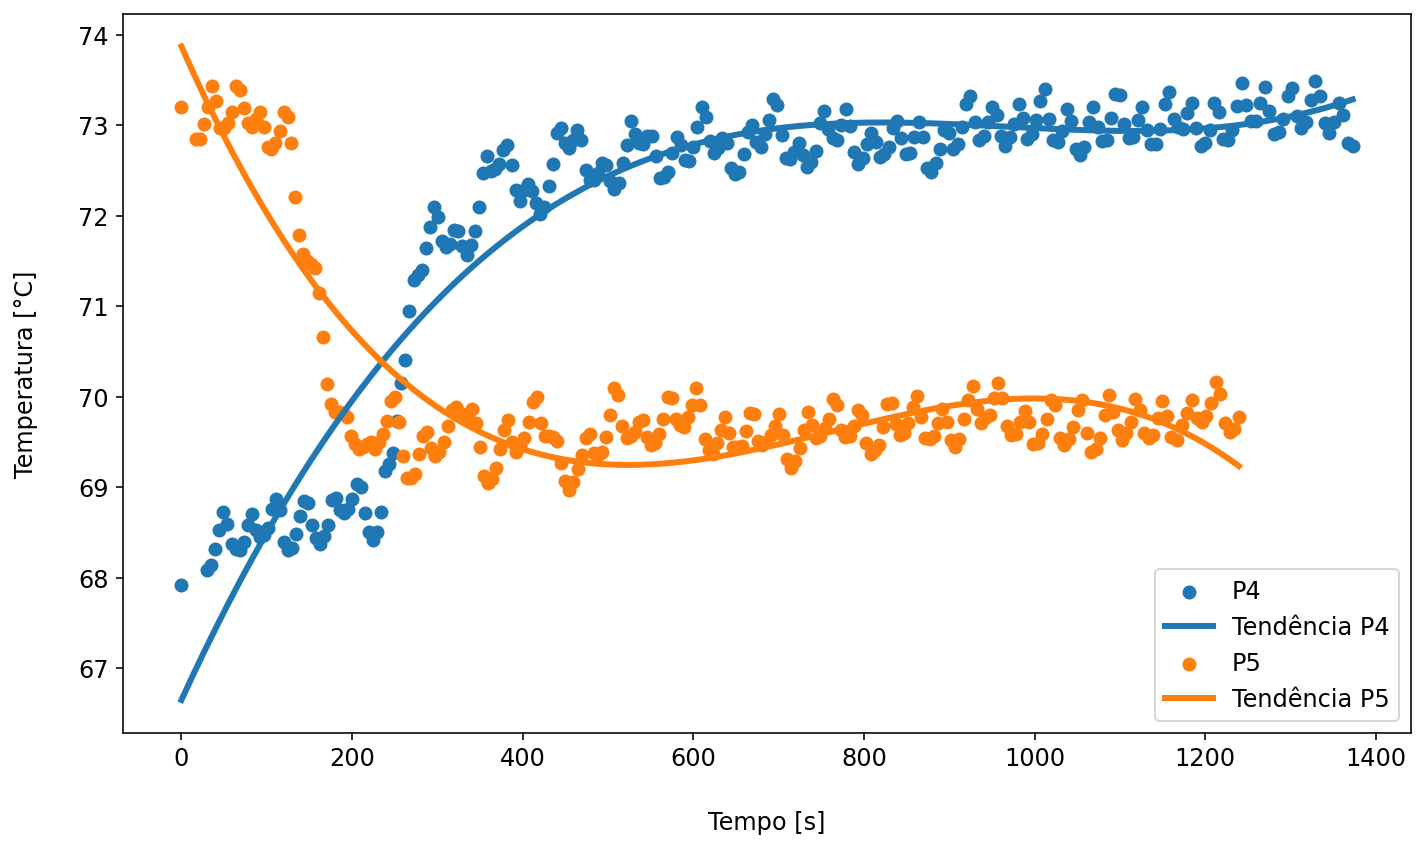
\includegraphics[width=1\linewidth]{FigurasdoTexto/Temperatura de Descargahyst.png}
    \caption{Temperatura de Descarga  nas Perturbações P4 e P5}
    \label{fig:TempDescargaSubidaeDescida}
    {\footnotesize Fonte: O Autor (2025)}
\end{figure}

A maior histerese encontrada nas variáveis de descarga, como observado na Figura \ref{fig:histereses normalizadas}, pode ser explicada pois estas variáveis são mais lentas em seu transiente, e são dependentes das variáveis de sucção e da ação da válvula de expansão, ou seja, elas acabam acumulando no seu resultado os efeitos da histerese destas outras partes do sistema. 

\subsection{\MakeUppercase{Análise do COP}}

Nesta subseção, serão apresentadas as análises do Coeficiente de Performance (COP) do sistema de condicionamento de ar nas condições de perturbação aplicadas ao sistema. O cálculo da determinação do COP foi feito conforme detalhado na subseção \ref{subsec:Determinação do COP do Sistema}.

\subsubsection{Efeito da Variação da Vazão de Ar do Ventilador no COP}

A capacidade de refrigeração do sistema oscila ao aumentar a vazão de ar do ventilador, o que é um resultado razoável devido ao analisado das perturbações nas temperaturas e pressões de sucção e descarga do compressor, analisadas com mais detalhe na subseção \ref{subsec:PertubaçãoVelVentilador}. A capacidade de refrigeração cresce e oscila com o aumento da vazão de ar do ventilador, isto é, para P1, como pode ser visto na Figura \ref{fig:Qe e W Perturbação Ventilador}. Isto ocorre devido, principalmente, à temperatura de saída e umidade relativa de saída do evaporador que apresentaram oscilações, o que afeta diretamente os cálculos de entalpia do ar. P3 oscila menos, o que deve estar relacionado com as razões explicadas anteriormente na subseção \ref{subsec:PertubaçãoVelVentilador}. A mudança abrupta capacidade de refrigeração ocorrem devido a mudança abrupta da vazão de ar do ventilador do evaporador.

\begin{figure}[h]
    \centering
    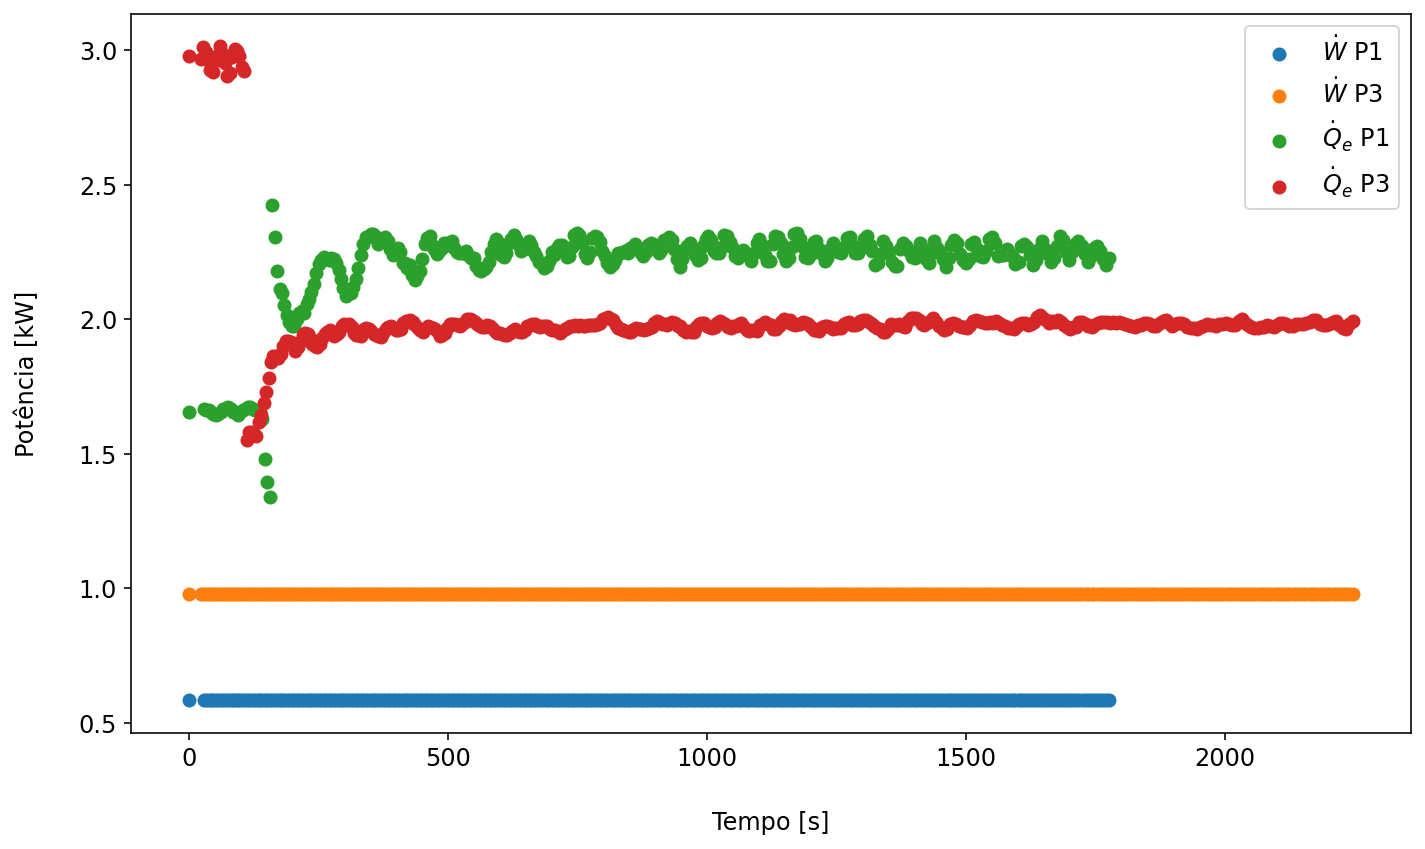
\includegraphics[width=1\linewidth]{FigurasdoTexto/Qe e W Perturbação Ventilador.png}
    \caption{Capacidade de Refrigeração e Potência Consumida Pelo Compressor nas Perturbações P1 e P3}
    \label{fig:Qe e W Perturbação Ventilador}
    {\footnotesize Fonte: O Autor (2025)}
\end{figure}

Portanto o COP também oscila, como pode ser visto na Figura \ref{fig:COP Perturbação Ventilador}. A oscilação do COP é completamente relacionada à oscilação da capacidade de refrigeração neste caso, já que a potência consumida pelo compressor é mantida fixa. Oscila para P1 e menos para P3. O COP cresce quando a vazão de ar aumenta e decresce quando ela diminui, tal resultado é aferido em outros estudos como, por exemplo, no artigo de \textcite{FanSpeedCOP-AlBadri} onde também foi observado que houve um aumento do COP ao aumentar a vazão de ar, caso a rotação do compressor seja mantida fixa. Este aumento ou diminuição do COP ocorre devido ao processo de troca de calor. Foi observado um aumento de 26\% no COP em P1 e redução de 33\% em P3, quando comparado ao estado estacionário.
\newpage
\begin{figure}[h]
    \centering
    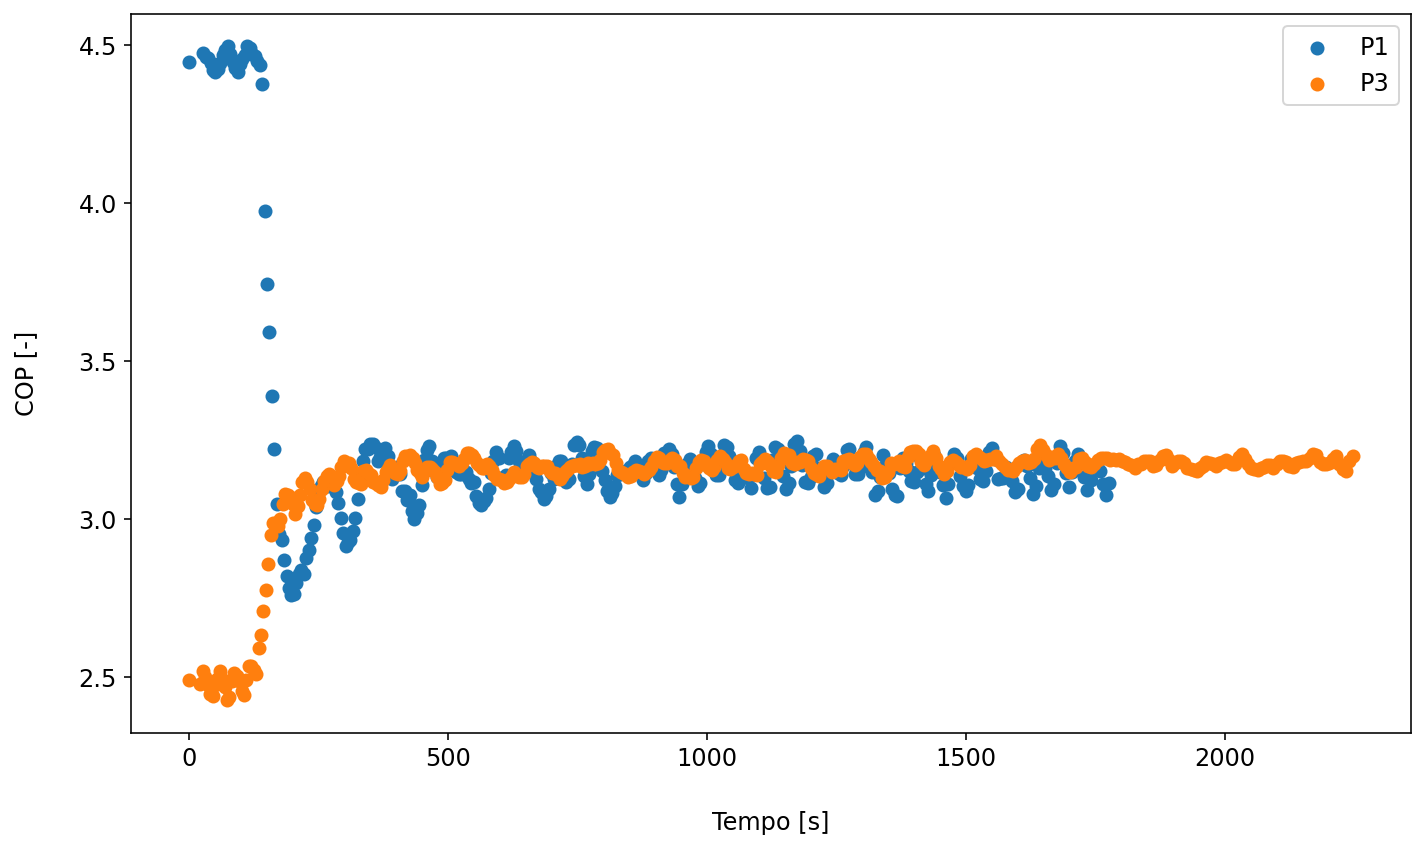
\includegraphics[width=1\linewidth]{FigurasdoTexto/COP Perturbação Ventilador.png}
    \caption{COP nas Perturbações P1 e P3}
    \label{fig:COP Perturbação Ventilador}
    {\footnotesize Fonte: O Autor (2025)}
\end{figure}

\subsubsection{Efeito da Variação de Rotação do Compressor no COP}

Nesta situação, ao aumentar a variação da rotação do compressor, a capacidade de refrigeração do sistema aumenta, como pode ser vista na Figura \ref{fig:Capacidade de Resfriamento e potência consumida pelo Compressor P2} para a perturbação P2. Isto ocorre devido à diminuição da entalpia de saída e ao aumento da entalpia de entrada do ar.
\newpage
\begin{figure}[h]
    \centering
    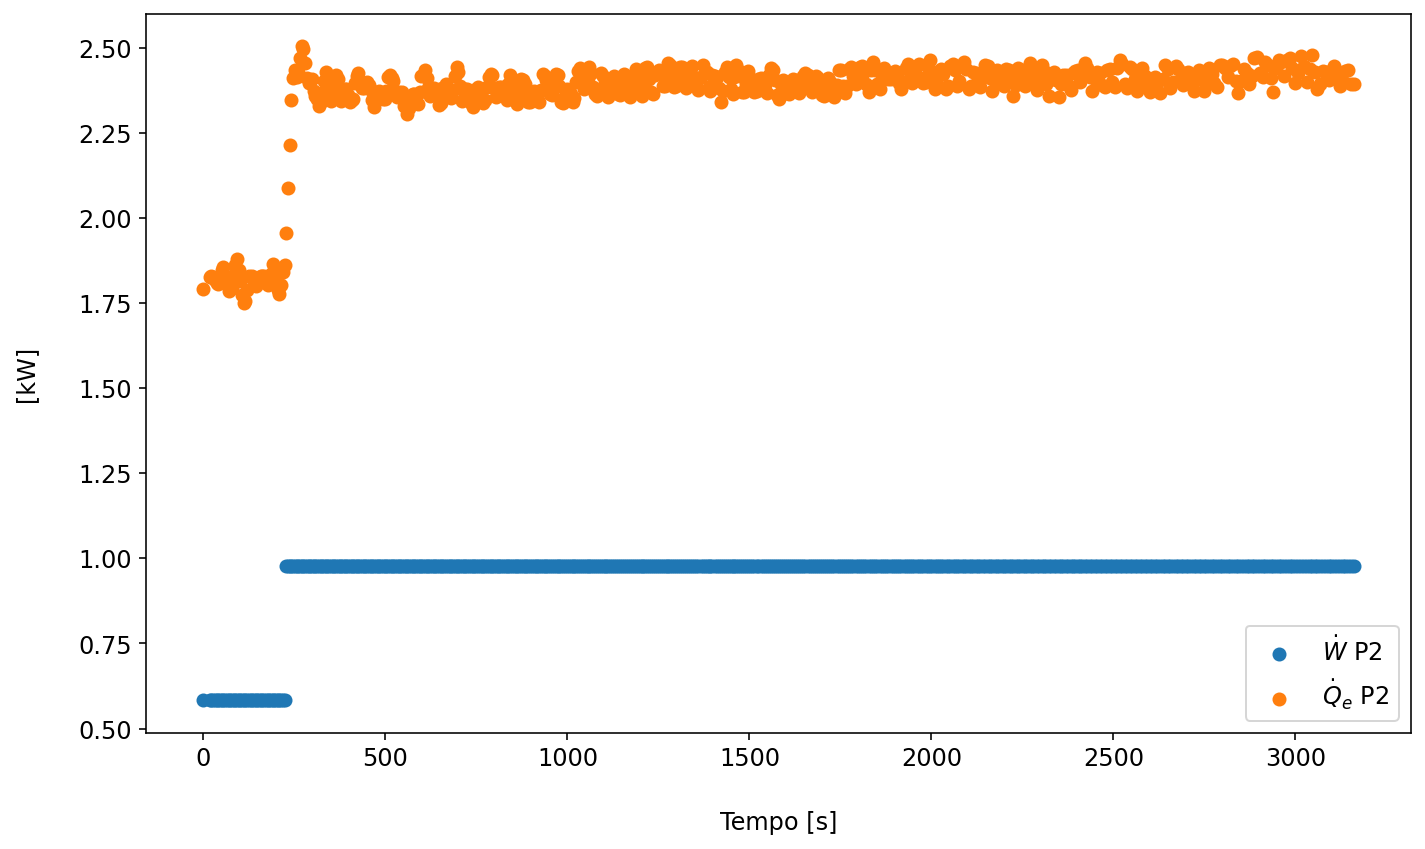
\includegraphics[width=1\linewidth]{FigurasdoTexto/Qe e W Perturbação Rot.png}
    \caption{Capacidade de Refrigeração e Potência Consumida Pelo Compressor na Perturbação P2}
    \label{fig:Capacidade de Resfriamento e potência consumida pelo Compressor P2}
    {\footnotesize Fonte: O Autor (2025)}
\end{figure}

É importante ressaltar que o transiente da potência consumida pelo compressor é, para efeitos práticos de análise, instantâneo, o que não acontece com a capacidade de refrigeração. Esta diferença entre os transientes da capacidade de refrigeração e da potência consumida pelo compressor pode ser vista na Figura \ref{fig:zoom capapcidade de refrigeração e potência de consumo}. O transiente imediato da potência consumida pelo compressor é o causador da variação abrupta do COP que pode ser observada nas Figuras \ref{fig:Análise do COP Rotação} e \ref{fig:Análise do COP Histerese} também. 
\newpage
\begin{figure}[h]
    \centering
    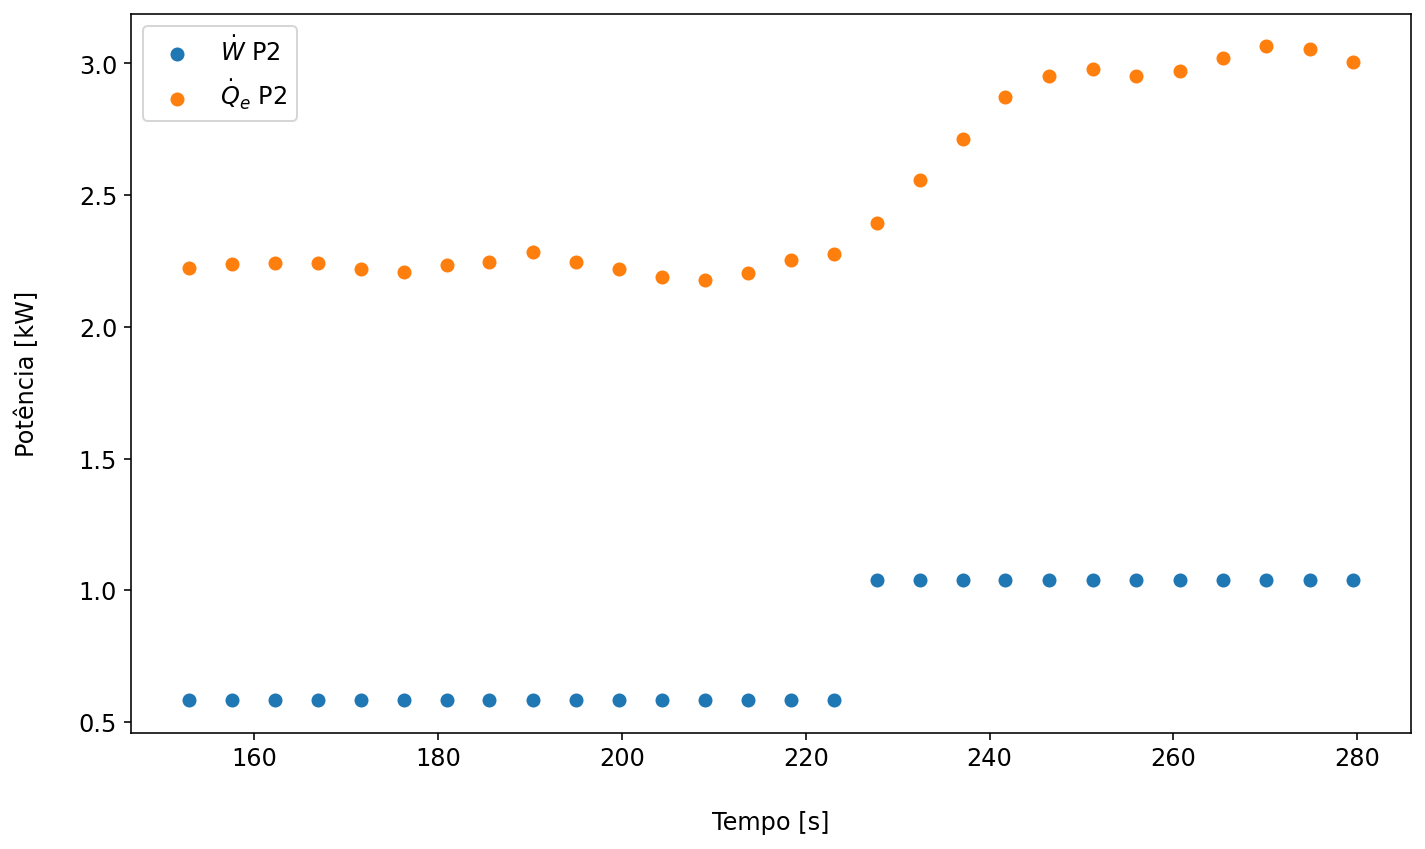
\includegraphics[width=1\linewidth]{FigurasdoTexto/Zoom Capacidade de Refrigeração e Potência de Consumo.png}
    \caption{Transiente da Capacidade de Refrigeração e Potência Consumida Pelo Compressor na Perturbação P2}
    \label{fig:zoom capapcidade de refrigeração e potência de consumo}
    {\footnotesize Fonte: O Autor (2025)}
\end{figure} 

Embora a capacidade de refrigeração do sistema aumente, o oposto ocorre no COP, como pode ser visto na Figura \ref{fig:Análise do COP Rotação}, o COP diminui com o aumento da rotação do compressor. Este resultado é bem documentado na literatura, por exemplo \textcite{MASCHE2021302} explica que o COP diminui devido ao aumento da potência consumida pelo compressor, aumentando mais do que a capacidade de refrigeração do sistema. Também pode estar atrelado às quedas de pressão do fluido refrigerante ao passar pelos trocadores de calor, como mencionado por \textcite{CONSTANTINO2022101048} o que pode levar à diminuição também da eficiência da compressão em rotações mais elevadas, como mencionado por \textcite{stoecker1998industrial}. Foi observada uma diminuição de 30\% no COP em P2, quando comparado ao estado estacionário.
\newpage
\begin{figure}[h]
    \centering
    \includegraphics[width=1\linewidth]{FigurasdoTexto/COP Perturbação Rot.png}
    \caption{COP na Perturbação P2}
    \label{fig:Análise do COP Rotação}
    {\footnotesize Fonte: O Autor (2025)}
\end{figure}

\subsubsection{Efeito da Histerese no COP}

Conforme \textcite{MASCHE2021302}, a influência da histerese no COP é muito mais dramática do que na capacidade de refrigeração do sistema. Isto acontece pois o trabalho de entrada de refrigeradores eficientes é muito baixo. O COP cai rapidamente e a histerese aumenta devido à redução da capacidade de refrigeração e ao aumento do trabalho de entrada do compressor. Esta frase é possível de ser verificada, para a capacidade de refrigeração, observando a Figura \ref{fig:Capacidade de Resfriamento e Potência de Entrada do Compressor P4 e P5}. Ela demonstra como a capacidade de refrigeração e a potência consumida pelo compressor variam nas perturbações P4 e P5. A potência consumida pelo compressor varia, para efeitos práticos, quase que instantaneamente, enquanto a capacidade de refrigeração varia de forma mais lenta e gradual, pois o transiente das entalpias está relacionado aos transientes de umidade e temperaturas do evaporador, que dependem também do restante do sistema, enquanto a rotação do compressor depende apenas do inversor.
\newpage
\begin{figure}[h]
    \centering
    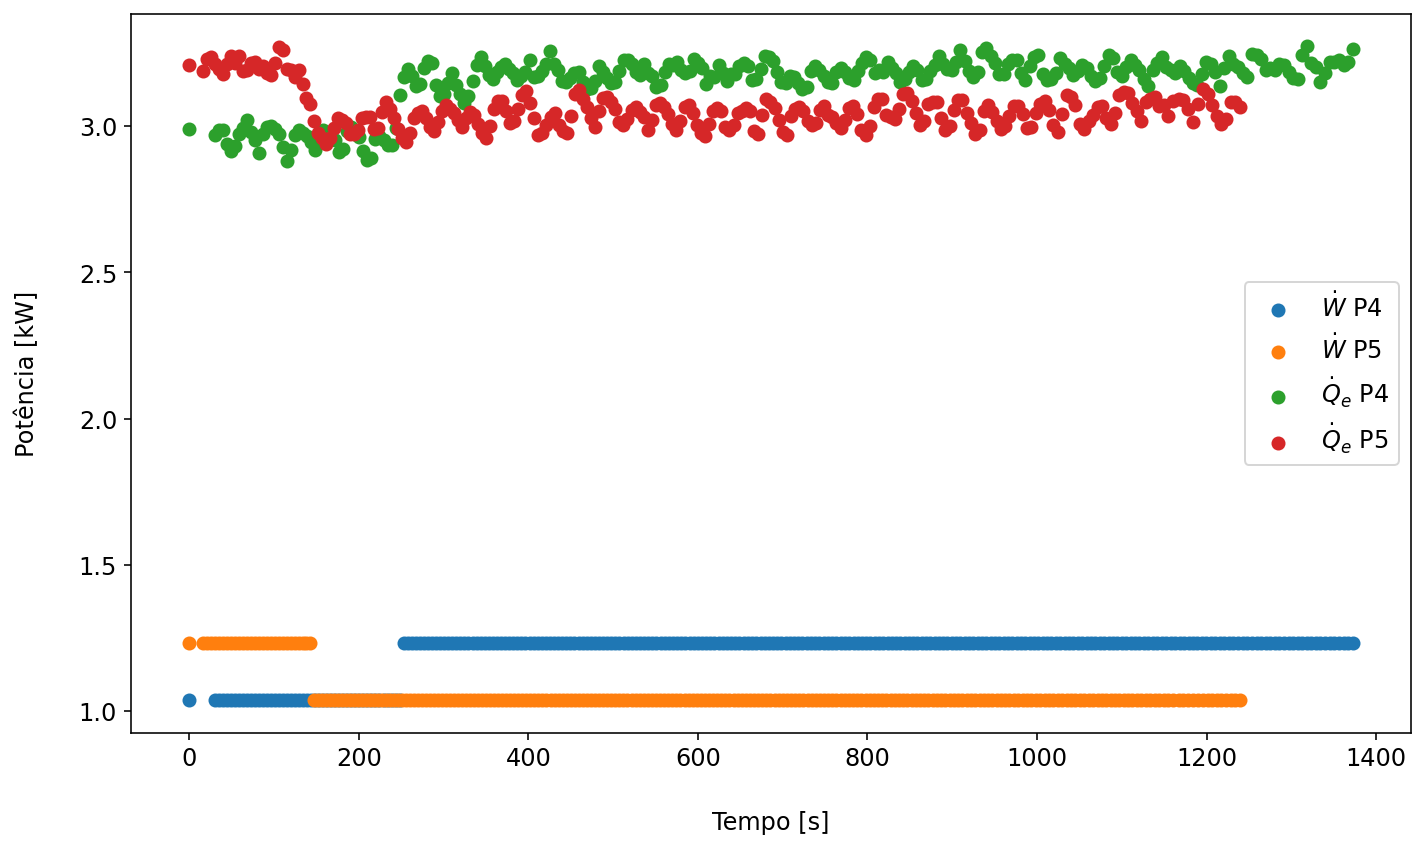
\includegraphics[width=1\linewidth]{FigurasdoTexto/Qe e W Histerese.png}
    \caption{Capacidade de Refrigeração e Potência Consumida Pelo Compressor nas Perturbações P4 e P5}
    \label{fig:Capacidade de Resfriamento e Potência de Entrada do Compressor P4 e P5}
    {\footnotesize Fonte: O Autor (2025)}
\end{figure}

Utilizando a equação \ref{eq:COP}, então é possível determinar o COP do sistema nas perturbações P4 e P5, o que pode ser visto na Figura \ref{fig:Análise do COP Histerese}, nota-se que a histerese do COP, como dito por \textcite{MASCHE2021302}, é acentuada e isso ocorre devido ao impacto da variação da potência consumida pelo compressor ser consideravelmente maior do que a variação da capacidade de refrigeração do sistema. A histerese normalizada do COP foi calculada como sendo 10\%, o que é um valor considerável. Houve também uma diminuição de 10\% no COP em P4 e 13\% de aumento em P5, quando comparado ao estado estacionário.
\newpage
\begin{figure}[h]
    \centering
    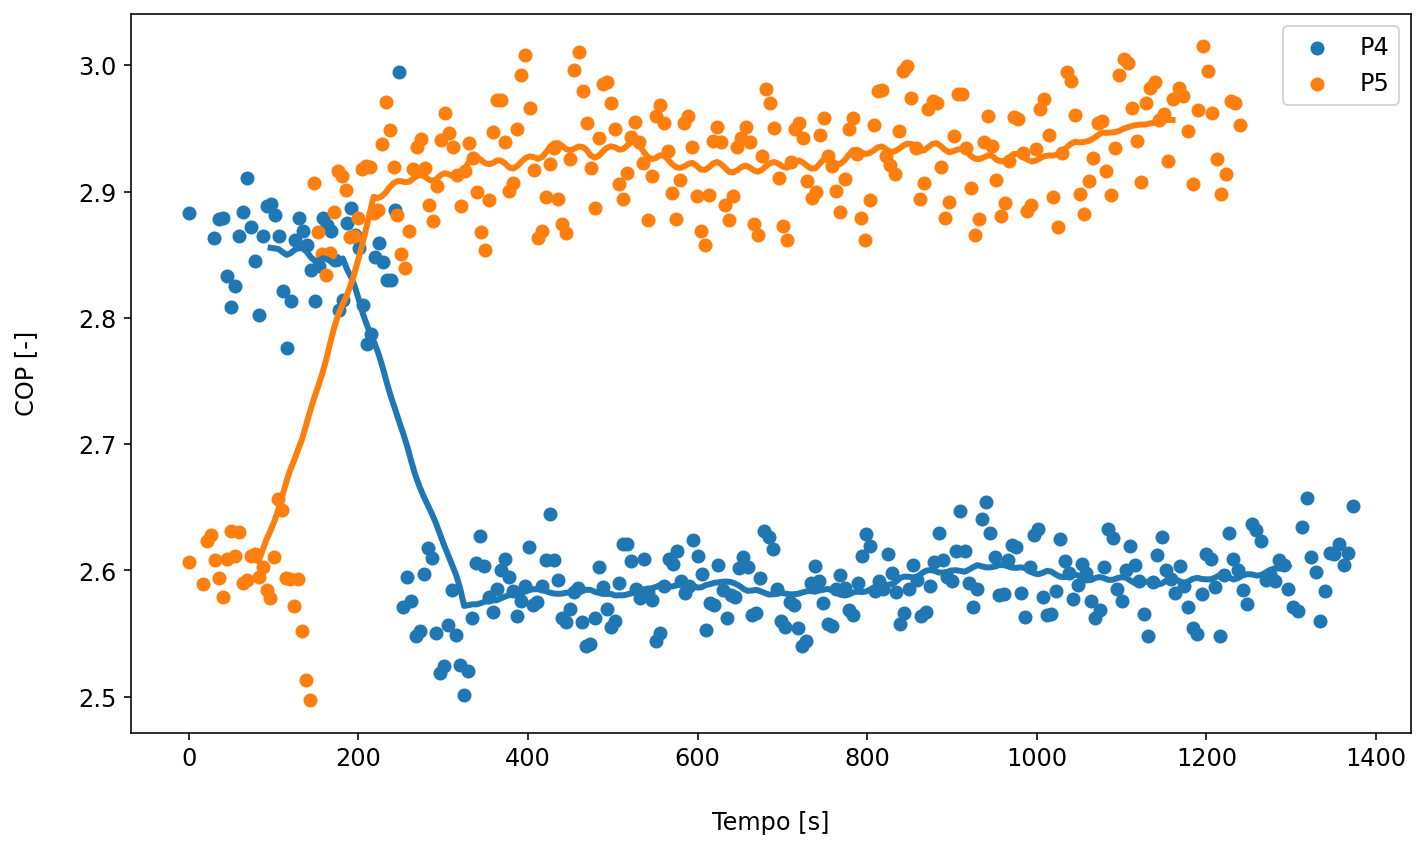
\includegraphics[width=1\linewidth]{FigurasdoTexto/COP Histerese1.png}
    \caption{Histerese no COP nas Perturbações P4 e P5}
    \label{fig:Análise do COP Histerese}
    {\footnotesize Fonte: O Autor (2025)}
\end{figure}

\subsection{\MakeUppercase{Estudo da Histerese Normalizada para Controle Não Adaptativo}}

Para finalizar esta seção, é interessante realizar um estudo final da histerese normalizada e estudar a relação dela com parâmetros do sistema, como, por exemplo, as suas constantes de tempo, que são um parâmetro importante e que são alteradas justamente devido à histerese do sistema.  

Todas as variáveis de teste aqui apresentadas, considerando as perturbações P4 e P5, podem ser consideradas, no tempo, como variáveis de primeira ordem, devido ao seu comportamento aproximadamente exponencial. Para tentar então encontrar a relação entre a histerese normalizada e as constantes de tempo do sistema, como a histerese é relativa à diferença entre os caminhos de subida e descida, então é proposto tentar encontrar uma relação entre a histerese normalizada e a diferença entre as constantes de tempo de subida e descida do sistema.
\newpage
A diferença entre as constantes de tempo do sistema pode ser então encontrada na Figura \ref{fig:Constantes de Tempo do Sistema}. As variáveis escolhidas para análise são as mesmas anteriormente apresentadas na Figura \ref{fig:histereses normalizadas}, sendo a única exceção a vazão de fluido refrigerante, já que ela não pode ser considerada de primeira ordem.

\begin{figure}[h]
    \centering
    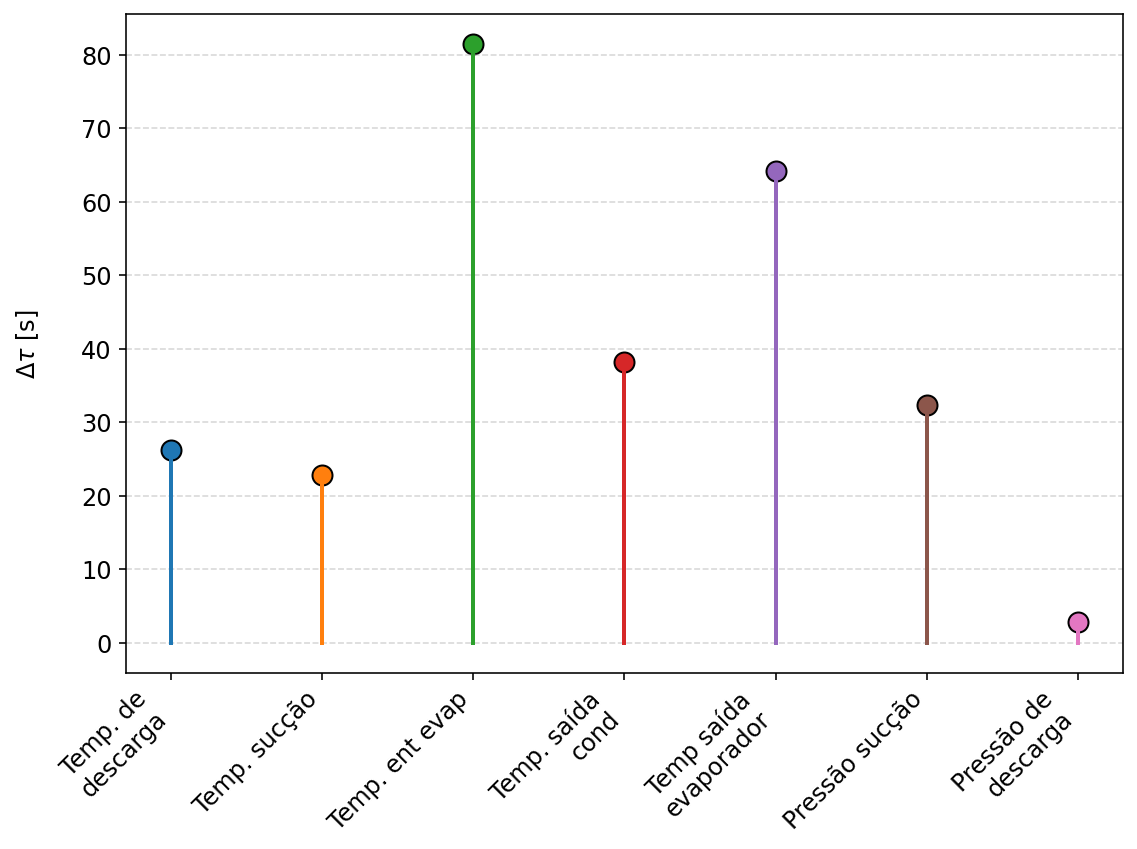
\includegraphics[width=1\linewidth]{FigurasdoTexto/Constantes de Tempo.png}
    \caption{Módulo da Diferença entre as Constantes de Tempo do Sistema nas Perturbações P4 e P5}
    \label{fig:Constantes de Tempo do Sistema}
    {\footnotesize Fonte: O Autor (2025)}
\end{figure}

 $\Delta \tau$ é o módulo da diferença entre as constantes de tempo de subida e descida do sistema, ou seja, $\Delta \tau = |\tau_{subida} - \tau_{descida}|$, onde $\tau_{subida}$ é a constante de tempo do sistema durante a subida da perturbação e $\tau_{descida}$ é a constante de tempo do sistema durante a descida da perturbação.

A partir dos dados apresentados na Figura \ref{fig:histereses normalizadas} e na Figura \ref{fig:Constantes de Tempo do Sistema}, é possível então traçar o gráfico da histerese normalizada pela diferença entre as constantes de tempo do sistema, como mostrado na Figura \ref{fig:HistNorm x Delta Tau}.

\newpage
\begin{figure}[h]
    \centering
    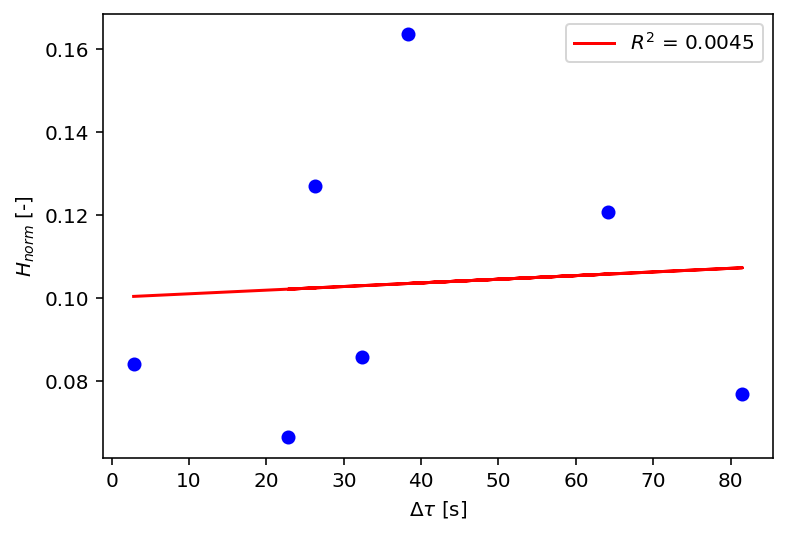
\includegraphics[width=1\linewidth]{FigurasdoTexto/HistNorm x Delta Tau.png}
    \caption{Histerese Normalizada e Módulo da Diferença entre as Constantes de Tempo do Sistema}
    \label{fig:HistNorm x Delta Tau}
    {\footnotesize Fonte: O Autor (2025)}
\end{figure}

Entretanto, não foi possível encontrar uma relação clara entre a histerese normalizada e a diferença entre as constantes de tempo do sistema. É possível notar que o R² da regressão linear entre a histerese normalizada e a diferença entre as constantes de tempo do sistema é baixo para tirar qualquer conclusão mais assertiva, indicando que a histerese normalizada parece não ter uma relação direta com a diferença entre as constantes de tempo do sistema, o que pode indicar que outros fatores estão influenciando a histerese do sistema.

Além desta análise, houve também a tentativa de encontrar uma relação linear entre o logaritmo da histerese normalizada e a diferença entre as constantes de tempo do sistema. A lógica por trás desta tentativa é que as funções de transferência de primeira ordem são exponenciais no domínio do tempo, o que poderia indicar então alguma relação linear entre os logaritmos da histerese normalizada e da diferença entre as constantes de tempo do sistema. No entanto, esta tentativa também não mostrou resultados satisfatórios, o que indica que talvez não seja possível encontrar uma relação direta entre a histerese normalizada e as constantes de tempo do sistema. 

Embora não tenha sido possível encontrar uma relação clara entre a histerese normalizada e as constantes de tempo do sistema, estes resultados obtidos não são inúteis em termos de controle.
Para um controle não adaptativo, saber a diferença entre as constantes de tempo pode ser bem útil para determinar o tempo de amostragem do controlador, ou seja, o tempo que o controlador deve esperar para fazer uma nova leitura das variáveis do sistema e tomar uma nova ação de controle. Isto é, escolher o menor tempo de amostragem possível para evitar que certas variáveis não sejam amostradas de maneira adequada, comprometendo o controle do sistema.

Todavia, é possível observar que há uma tendência geral de que quanto maior a diferença entre as constantes de tempo do sistema, maior é a histerese normalizada. Isto, embora não funcionará nessariamente em todos os casos, pode ser utilizado como uma regra prática para realizar certos cuidados no projeto do controlador para lidar com uma possível alta histerese no sistema.

Também vê-se necessário que o controlador seja projetado de tal forma que tenha uma banda morta em torno do valor de referência desejado, isto porque é possível que os valores em estado estacionário do sistema da ida não sejam exatamente iguais aos da volta, assim como observado na Figura \ref{fig:TempDescargaSubidaeDescida}. É importante então que o controlador entenda que uma certa variação em torno do valor de referência é aceitável, e que não deve ser considerado um erro de controle, mas sim uma característica do sistema.

Por fim, para um controle adaptativo, é possível utilizar modelos matemáticos mais complexos para modelar o fenômeno da histerese do sistema de forma mais precisa. Um exemplo de modelo que poderia ser utilizado é o modelo de histerese de Bouc-Wen, que é um modelo matemático não linear que pode ser utilizado para modelar sistemas com histerese, como utilizado por \textcite{ZHANG2024112387}. Neste artigo, foi utilizado para modelar histerese em um sistema de servoacionamento de microdeslocamento piezolétrico. Obtendo erro máximo de 0,06\% em uma trajetória senoidal, o que demonstra que esta abordagem pode ser bastante eficaz para modelar sistemas com histerese e, se necessário, pode ser utilizada para projetar um controlador adaptativo para um sistema de condicionamento de ar. Além do modelo de Bouc-Wen, o modelo de Prandtl-Ishlinskii também é um modelo matemático que pode ser utilizado para modelar sistemas com histerese, porém, conforme também \textcite{ZHANG2024112387}, ele é computacionalmente mais complexo que o de Bouc-Wen. Mesmo assim, pode ser interessante de ser utilizado em estudos futuros.



%Adicionar relação entre os taus do sistema de primeira ordem e a histerese normalizada, verifica se há e se sim qual a relação (gráfico de histnorm vs tau)


%Finalizar recomendando um plano de controle para caso não haja um controle adaptativo escolher se é melhor fazer pela subida ou pela descida.$\tau$